\input{"preamble.tex"}

\addbibresource{Precalculus.bib}

\let\Begin\begin
\let\End\end
\newcommand\wrapenv[1]{#1}

\makeatletter
\def\ScaleWidthIfNeeded{%
 \ifdim\Gin@nat@width>\linewidth
    \linewidth
  \else
    \Gin@nat@width
  \fi
}
\def\ScaleHeightIfNeeded{%
  \ifdim\Gin@nat@height>0.9\textheight
    0.9\textheight
  \else
    \Gin@nat@width
  \fi
}
\makeatother

\setkeys{Gin}{width=\ScaleWidthIfNeeded,height=\ScaleHeightIfNeeded,keepaspectratio}%

\title{
\rule{\linewidth}{1pt} \\
\textbf{
    Precalculus
  }
    \\ {\normalsize University of Georgia, Spring 2021} \\
  \rule{\linewidth}{2pt}
}
\titlehead{
    \begin{center}
  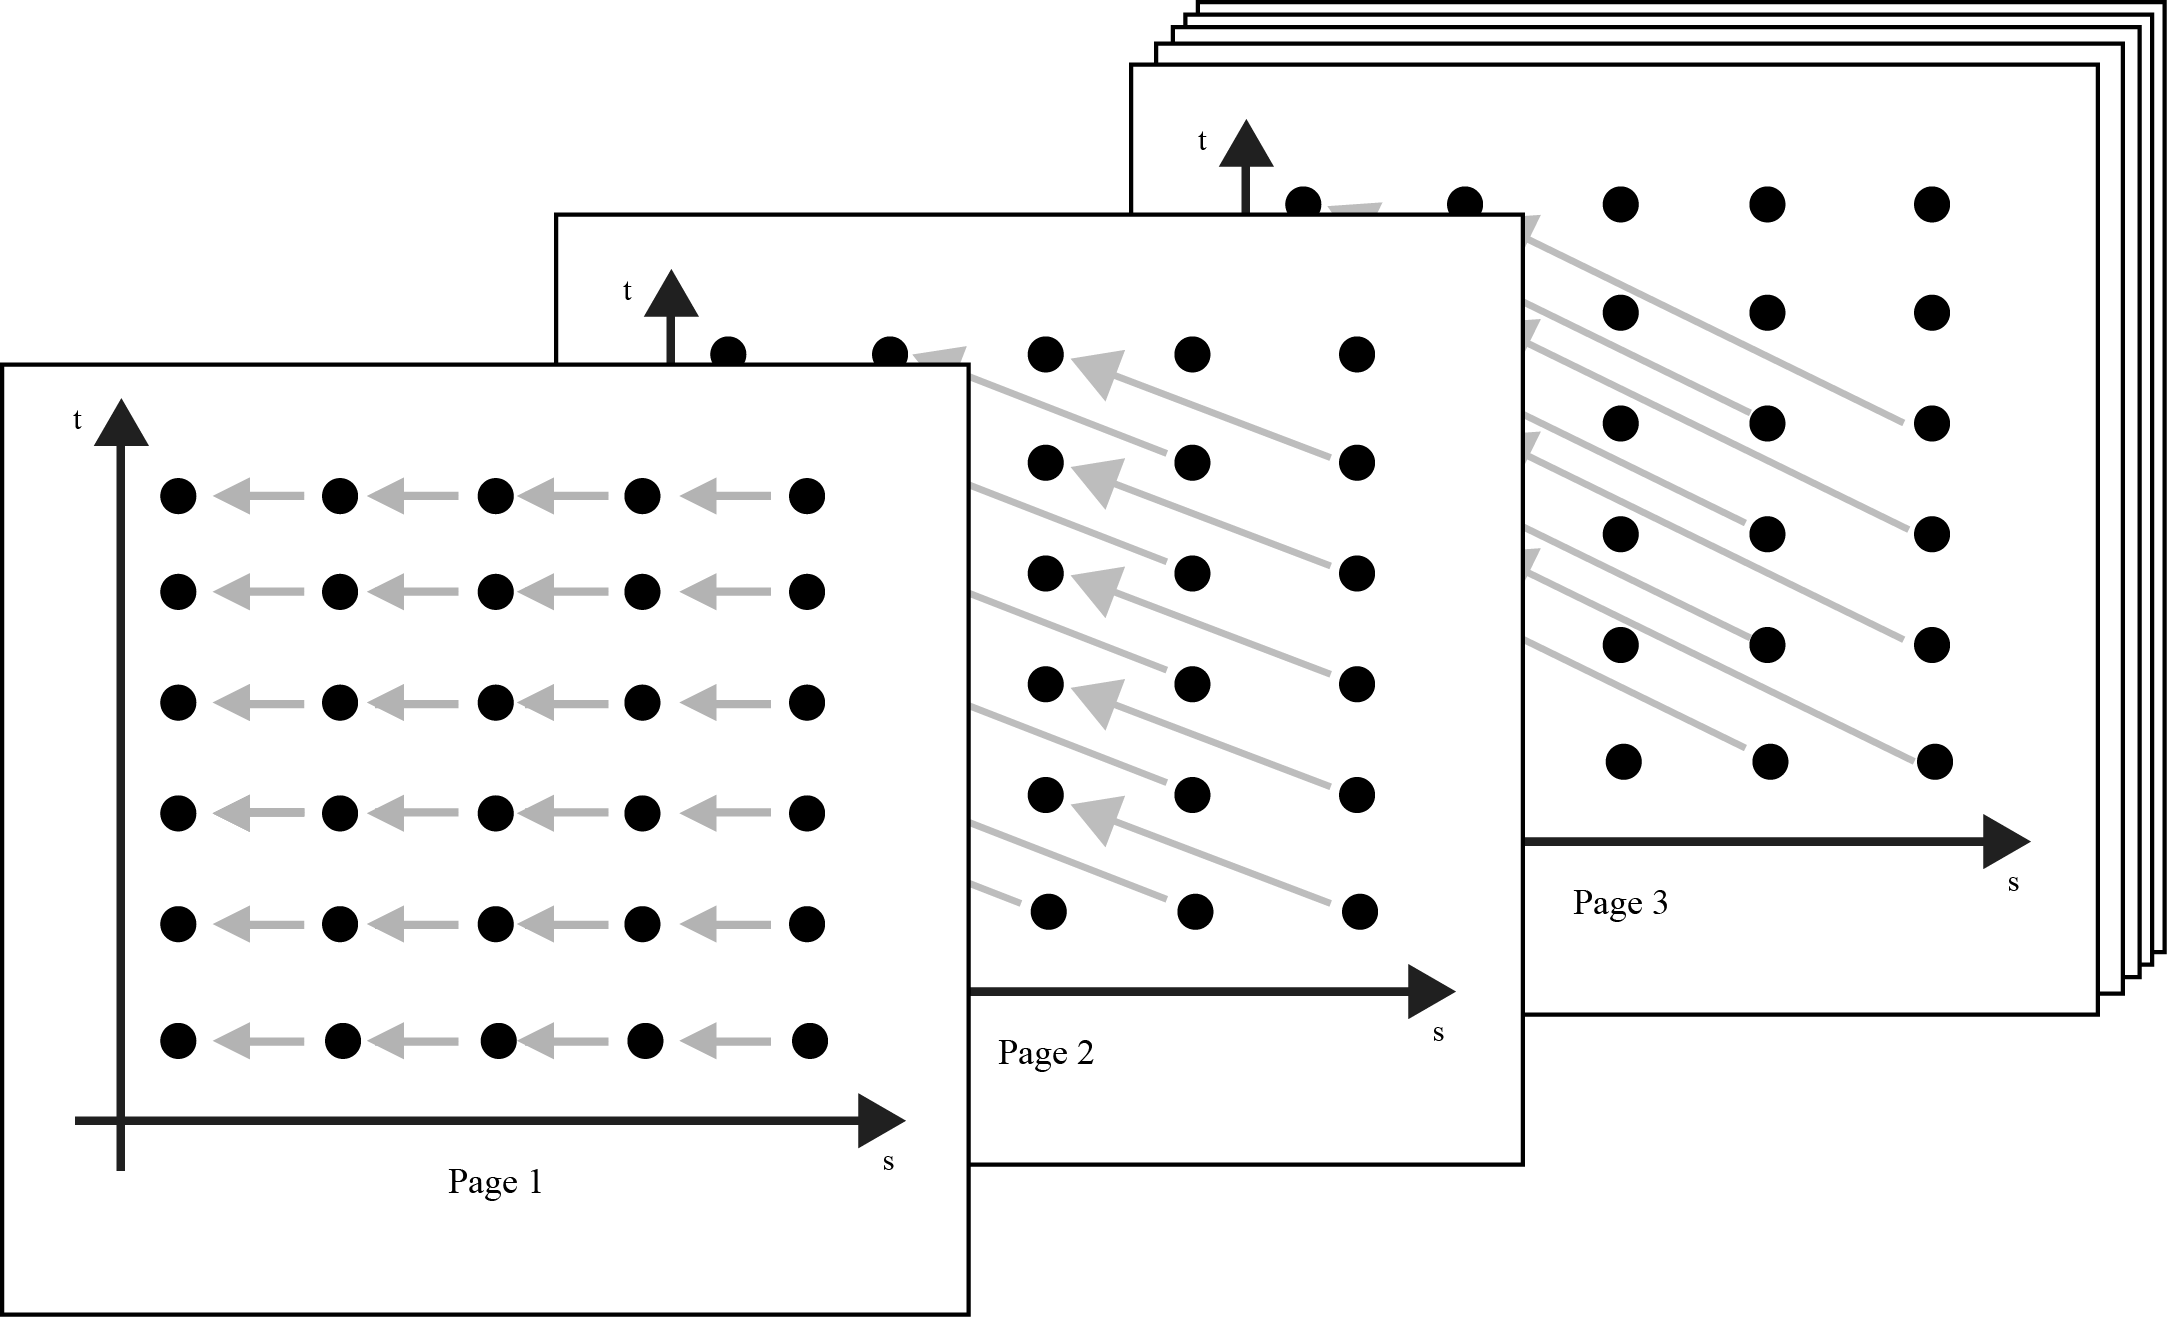
\includegraphics[width=\linewidth,height=0.45\textheight,keepaspectratio]{figures/cover.png}
  \end{center}
       \begin{minipage}{.35\linewidth}
    \begin{flushleft}
      \vspace{2em}
      {\fontsize{6pt}{2pt} \textit{Notes: These are rough notes for the
Math 1113 Precalculus course at the University of Georgia } } \\
    \end{flushleft}
    \end{minipage}
    \hfill
    \begin{minipage}{.65\linewidth}
    \end{minipage}
  }







\begin{document}

\date{}
\author{D. Zack Garza}
\maketitle
\begin{flushleft}
\textit{D. Zack Garza} \\
\textit{University of Georgia} \\
  \textit{\href{mailto: dzackgarza@gmail.com}{dzackgarza@gmail.com}} \\
{\tiny \textit{Last updated:} 2021-04-22 }
\end{flushleft}


\newpage

% Note: addsec only in KomaScript
\addsec{Table of Contents}
\tableofcontents
\newpage

\hypertarget{preface}{%
\section{Preface}\label{preface}}

\hypertarget{unit-1-functions}{%
\section{Unit 1: Functions}\label{unit-1-functions}}

\begin{theorem}[The Pythagorean Theorem]

If \(a,b\) are the legs of a right triangle with hypotenuse \(c\), there
is a relation
\begin{align*}
a^2 + b^2 = c^2
.\end{align*}

\end{theorem}

\begin{theorem}[The Distance Formula]

If \(p = (x_1, y_1)\) and \(q = (x_2, y_2)\) are points in the Cartesian
plane, then there is a \textbf{distance function}
\begin{align*}
d: \left\{{ \text{Pairs of points } (p, q) }\right\} \to {\mathbb{R}}\\
(p, q) &\mapsto d(p, q) \coloneqq\sqrt{ (x_2 - x_1)^2 + (y_2 - y_q)^2}
.\end{align*}

\end{theorem}

\todo[inline]{Law of cosines}

\begin{definition}[Linear Functions]

A function \(f:{\mathbb{R}}\to {\mathbb{R}}\) is \textbf{linear} if and
only if \(f\) has a formula of the following form:
\begin{align*}
f(x) = \alpha x + \beta && \alpha, \beta \in {\mathbb{R}}
.\end{align*}

\end{definition}

\begin{definition}[Intercepts]

Given a function \(f: {\mathbb{R}}\to {\mathbb{R}}\), an
\textbf{\(x{\hbox{-}}\)intercept} of \(f\) is a point \((x_0, 0)\) on
the graph of \(f\), so \(f(x_0) = 0\). Equivalently, it is a point on
the intersection of the graph and the \(x{\hbox{-}}\)axis.

\hfill\break

A \textbf{\(y{\hbox{-}}\)intercept} of \(f\) is a point \((0, y_0)\) on
the graph of \(f\), so \(f(0) = y_0\). Equivalently, it is a point on
the intersection of the graph and the \(y{\hbox{-}}\)axis.

\end{definition}

\begin{definition}[Relation]

A \textbf{relation} on two sets \(X\) and \(Y\) is a set of ordered
pairs \((x, y) \in X \times Y\), so \(R\) can be described as a set:
\begin{align*}
R = \left\{{ (x_0, y_0), (x_1, y_2), \cdots }\right\} 
.\end{align*}

The \textbf{domain} of the relation is the set of all \(x\in X\) that
occur in the first slot of these pairs, and the \textbf{range} is the
set of all \(y\in Y\) that occur in the second slot.

\end{definition}

\begin{definition}[Function]

A relation \(R\) is a \textbf{function} if it satisfies the following
\emph{deterministic property}: for every
\(x_0\in \operatorname{dom}(R)\), there is exactly \emph{one} pair of
the form \((x_0, y_0) \in R\).

\end{definition}

\begin{remark}

This says we can think of \(X\) as ``inputs'' and \(Y\) as ``output'',
and a function is a way to unambiguously assign inputs to outputs. It
can be useful to think of functions like programs: if I send in an
\(x\), what \(y\) should the program return to me? If I run this program
today, tomorrow, and 100 years from now, sending in the same \(x\) every
time, we might want it to give the same output every time, which is the
\emph{deterministic} property: I can \emph{determine} a single unique
output if I know what the input is. If my program tells me that
\(2+2=4\) today but \(2+2=5\) tomorrow, who knows what it will return in
100 years! We can't ``determine'' it.

\end{remark}

\begin{slogan}

For domains and ranges:

\begin{itemize}
\tightlist
\item
  Domains: the set of \emph{meaningful} inputs that the function
  ``knows'' how to handle.
\item
  Ranges: the set of \emph{attainable} outputs that we can expect.
\end{itemize}

\end{slogan}

\begin{remark}

To determine a domain:

\begin{enumerate}
\def\labelenumi{\arabic{enumi}.}
\tightlist
\item
  Naively hope it is \emph{all} of \({\mathbb{R}}\).
\item
  Throw out ``problematic'' points.
\item
  Draw a number line and write out what you are left with in interval
  notation.
\end{enumerate}

\end{remark}

\begin{example}[?]

Define
\begin{align*}
f: {\mathbb{R}}&\to {\mathbb{R}}\\
x &\mapsto {1\over x}
.\end{align*}

Then
\(\operatorname{dom}(f) = {\mathbb{R}}\setminus\left\{{0}\right\}= (-\infty, 0) \cup(0, \infty)\)
and \(\mathop{\mathrm{range}}(f) = {\mathbb{R}}\).

\end{example}

\begin{example}[?]

Define
\begin{align*}
f: {\mathbb{R}}&\to {\mathbb{R}}\\
x &\mapsto \sqrt{x}
.\end{align*}

Then
\(\operatorname{dom}(f) = {\mathbb{R}}\setminus(-\infty, 0) = [0, \infty)\)
and \(\mathop{\mathrm{range}}(f) = [0, \infty)\).

\end{example}

\hypertarget{unit-2-exponential-and-logarithmic-functions}{%
\section{Unit 2: Exponential and Logarithmic
Functions}\label{unit-2-exponential-and-logarithmic-functions}}

\hypertarget{unit-3-trigonometric-functions}{%
\section{Unit 3: Trigonometric
Functions}\label{unit-3-trigonometric-functions}}

\hypertarget{general-notes}{%
\subsection{General Notes}\label{general-notes}}

\begin{itemize}
\item
  In this section, always draw a picture! Virtually 100\% of the time.

  \begin{itemize}
  \tightlist
  \item
    In particular, a unit circle should almost always show up.
  \end{itemize}
\item
  Use exact ratios wherever possible.
\item
  There are too many details and formulas to just memorize in this unit:
  focus on the \textbf{processes}.
\end{itemize}

\hypertarget{common-mistakes}{%
\subsection{Common Mistakes}\label{common-mistakes}}

Some facts to remember:

\begin{itemize}
\tightlist
\item
  \(\sin^{-1}(\theta) \neq 1/\sin(\theta)\). Mnemonic: reciprocals of
  trigonometric functions already have a better name, here
  \(\csc(\theta)\).
\end{itemize}

\hypertarget{basic-trigonometric-functions}{%
\subsection{Basic Trigonometric
Functions}\label{basic-trigonometric-functions}}

\todo[inline]{Sin/cos/etc as ratios}

\hypertarget{proportionality-relationships}{%
\subsection{Proportionality
Relationships}\label{proportionality-relationships}}

\begin{definition}[Radian]

\todo[inline]{What is a 1 radian?}

\begin{figure}
\centering
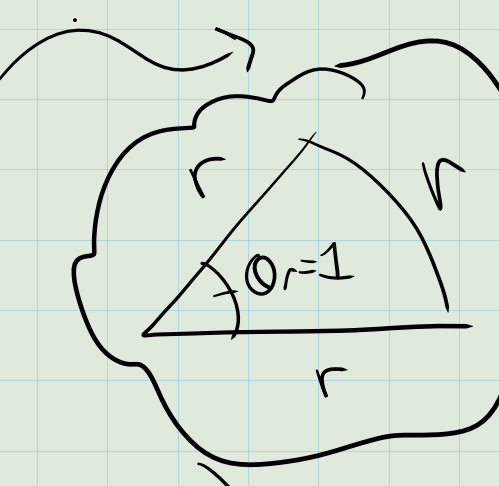
\includegraphics{figures/image_2021-04-18-21-51-59.png}
\caption{image\_2021-04-18-21-51-59}
\end{figure}

\end{definition}

\begin{remark}

In geometric terms, an angle in radians in the ratio of the arc length
\(s(\theta, R)\) to the radius \(R\), so
\begin{align*}
\theta_R = {s(\theta, R) \over R}
.\end{align*}

\end{remark}

\begin{definition}[Coterminal Angles]

If \(\theta\) is an abstract angle, we will say
\(\theta + k\,\text{rev} \simeq \theta\) for any integer
\(k\in {\mathbb{Z}}\). Any such angle is said to be \textbf{coterminal}
to \(\theta\).

\end{definition}

\begin{remark}

In radians:
\begin{align*}
\theta_R \simeq \theta_R + k\cdot 2\pi && k\in {\mathbb{Z}}
.\end{align*}

In degrees:
\begin{align*}
\theta_D \simeq \theta_D + k\cdot 360^\circ && k\in {\mathbb{Z}}
.\end{align*}

\end{remark}

\begin{proposition}[Degrees are related to radians]

\todo[inline]{todo}

\begin{align*}
{\theta \over 1\,\text{rev}} = {\theta_R \over 2\pi\, \text{rad} } = {\theta_D \over 360^\circ}
.\end{align*}

\end{proposition}

\begin{proposition}[Arc length and sector area are related to radians]

\todo[inline]{todo}

\begin{align*}
{\theta \over 1\,\text{rev}}
= 
{s(R, \theta) \over 2\pi R} 
= 
{ A(R, \theta) \over \pi R^2 }
.\end{align*}

This implies that
\begin{align*}
A(R, \theta) &={R^2 \theta \over 2} \\
s(R, \theta) &= R\theta
.\end{align*}

\end{proposition}

\hypertarget{trigonometric-functions-as-ratios}{%
\subsection{Trigonometric Functions as
Ratios}\label{trigonometric-functions-as-ratios}}

\begin{definition}[?]

There are 6 trigonometric functions defined by the following ratios:

\todo[inline]{soh-cah-toa, cho-sha-cao}

\end{definition}

\begin{proposition}[Domains of trigonometric functions]

\begin{longtable}[]{@{}
  >{\raggedright\arraybackslash}p{(\columnwidth - 4\tabcolsep) * \real{0.20}}
  >{\raggedright\arraybackslash}p{(\columnwidth - 4\tabcolsep) * \real{0.64}}
  >{\raggedright\arraybackslash}p{(\columnwidth - 4\tabcolsep) * \real{0.14}}@{}}
\toprule
Function & Domain & Range \\
\midrule
\endhead
\(\sin\) & \({\mathbb{R}}\) & \([-1, 1]\) \\
\(\cos\) & \({\mathbb{R}}\) & \([-1, 1]\) \\
\(\tan\) &
\({\mathbb{R}}\setminus\left\{{\pm {\pi \over 2}, \pm{3\pi \over 2}, \cdots}\right\}\)
& ? \\
\(\csc\) &
\({\mathbb{R}}\setminus\left\{{0, \pm {\pi}, \pm{2\pi}, \cdots}\right\}\)
& ? \\
\(\sec\) &
\({\mathbb{R}}\setminus\left\{{\pm {\pi \over 2}, \pm{3\pi \over 2}, \cdots}\right\}\)
& ? \\
\(\cot\) &
\({\mathbb{R}}\setminus\left\{{0, \pm {\pi}, \pm{2\pi}, \cdots}\right\}\)
& ? \\
\bottomrule
\end{longtable}

\end{proposition}

\hypertarget{polar-coordinates}{%
\subsection{Polar Coordinates}\label{polar-coordinates}}

\begin{definition}[Unit Circle]

The \textbf{unit circle} is defined as
\begin{align*}
S^1 \coloneqq\left\{{ \mathbf{p} = (x, y) \in {\mathbb{R}}^2 {~\mathrel{\Big|}~}d(\mathbf{p}, \mathbf{0}) = 1 }\right\} = \left\{{ (x, y) \in {\mathbb{R}}^2 {~\mathrel{\Big|}~}x^2 + y^2 = 1 }\right\} 
,\end{align*}
the set of all points in the plane that are distance exactly 1 from the
origin.

\end{definition}

\begin{theorem}[Polar Coordinates]

If a vector \(\mathbf{v}\) has at an angle of \(\theta\) in radians and
has length \(R\), the corresponding point \(\mathbf{p}\) at the end of
\(\mathbf{v}\) is given by
\begin{align*}
\mathbf{p} = {\left[ {x, y} \right]} = {\left[ {R\cos(\theta), R\sin(\theta)} \right]}
.\end{align*}

Conversely, if \((x, y)\) are known, then the corresponding \(R\) and
\(\theta\) are given by
\begin{align*}
[R, \theta] = {\left[ { \sqrt{x^2 + y^2}, \arctan\qty{y\over x} } \right]}
.\end{align*}

\end{theorem}

\begin{corollary}[Polar Coordinates on $S^1$]

If \(R=1\), so \(\mathbf{v}\) is on the unit circle \(S^1\), then
\begin{align*}
[x, y] = [\cos(\theta), \sin(\theta)]
.\end{align*}

\end{corollary}

\begin{remark}

This is a very important fact! The \(x, y\) coordinates on the unit
circle \emph{literally} corresponding to cosines and sines of subtended
angles will be used frequently.

\end{remark}

\begin{slogan}

Cosines are like \(x\) coordinates, sines are like \(y\) coordinates.

\end{slogan}

\begin{example}[?]

Given \(\theta_R = 4\pi/3\), what is the corresponding point on the unit
circle \(S^1\)?

\end{example}

\begin{warnings}

Note that \(\sin(\theta), \cos(\theta)\) work for any \(\theta\) at all.
However, \(\cos(\theta) = 0\) sometimes, so
\(\tan(\theta) \coloneqq\sin(\theta) / \cos(\theta)\) will on occasion
be problematic. Similar story for the other functions.

\end{warnings}

\hypertarget{special-angles}{%
\subsection{Special Angles}\label{special-angles}}

For reference: the unit circle.
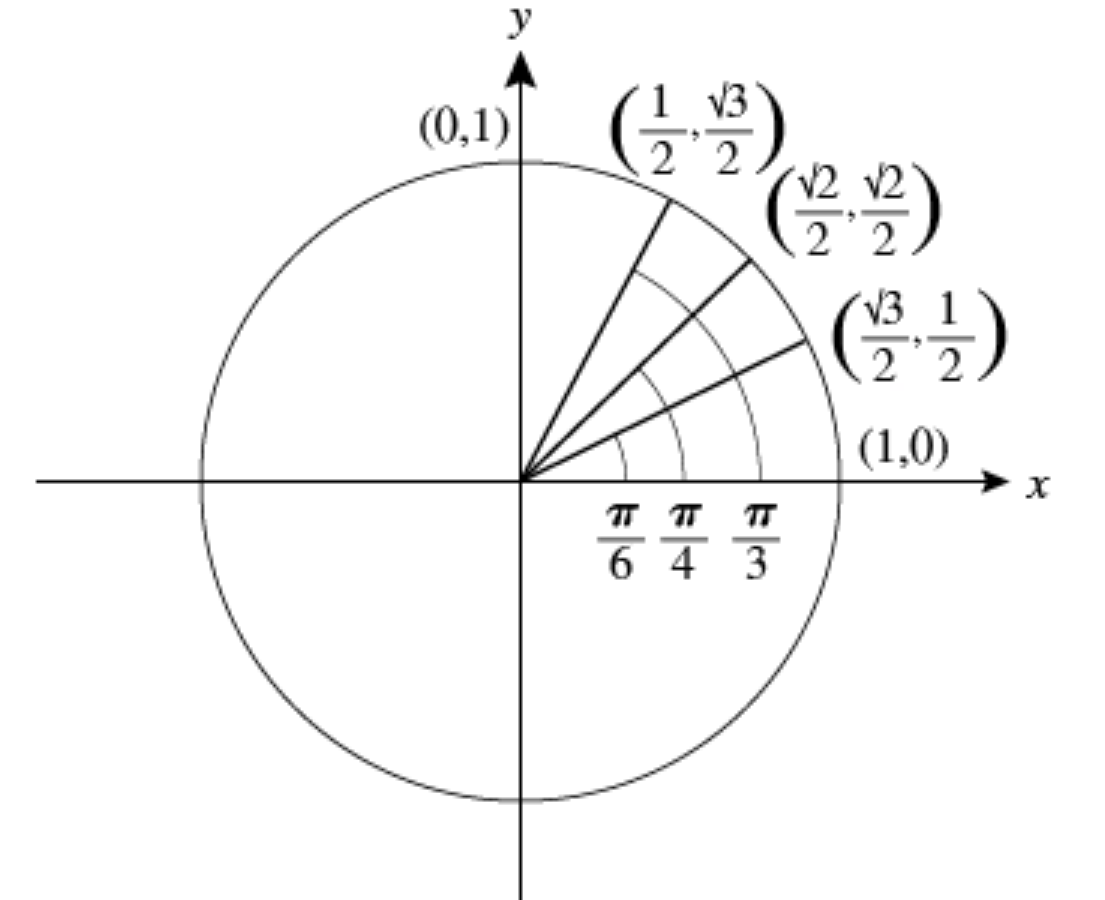
\includegraphics{figures/image_2021-04-18-21-06-45.png}

\begin{remark}

Idea: we want to partition the circle simultaneously

\begin{itemize}
\tightlist
\item
  Into 8 pieces, so we increment by \(2\pi/8 = \pi/4\)
\item
  Into 12 pieces, so we increment by \(2\pi/12 = \pi/6\).
\end{itemize}

\end{remark}

\begin{proposition}[Trick to memorize special angles]

\todo[inline]{Table of special angles, increasing/decreasing}

\end{proposition}

\hypertarget{reference-angles-and-the-flipping-method}{%
\subsection{Reference Angles and the Flipping
Method}\label{reference-angles-and-the-flipping-method}}

\begin{definition}[Reference Angle]

Given a vector at of length \(R\) and angle \(\theta\), the
\textbf{reference angle} \({ \theta_{\mathrm{Ref} } }\) is the acute
angle in the triangle formed by dropping a perpendicular to the nearest
horizontal axis.

\end{definition}

\begin{proposition}[?]

Reference angles for each quadrant:
\begin{align*}
\text{Quadrant II}: && \theta + { \theta_{\mathrm{Ref} } }= \pi \\
\text{Quadrant III}: && \pi + { \theta_{\mathrm{Ref} } }= \theta \\
\text{Quadrant IV}: && \theta + { \theta_{\mathrm{Ref} } }= 2\pi
.\end{align*}

\end{proposition}

\begin{example}[?]

Given \(\sin(\theta) = 7/25\), what are the five remaining trigonometric
functions of \(\theta\)?

Method:

\begin{enumerate}
\def\labelenumi{\arabic{enumi}.}
\tightlist
\item
  Draw a picture! Embed \(\theta\) into a right triangle.
\item
  Find the missing side using the Pythagorean theorem.
\item
  Use definition of trigonometric functions are ratios.
\end{enumerate}

\end{example}

\begin{remark}

Note that you can not necessarily find the angle \(\theta\) here, but we
didn't need it. If we \emph{did} want \(\theta\), we would need an
inverse function to free the argument:
\begin{align*}
\sin(\theta) &= 7/25 \\
\implies \arcsin( \sin(\theta) ) = \arcsin(7/25) \\
\implies \theta = \arcsin(7/25) \\
.\end{align*}

\end{remark}

\hypertarget{identities-using-pythagoras}{%
\subsection{Identities Using
Pythagoras}\label{identities-using-pythagoras}}

\begin{proposition}[?]

\begin{align*}
(\sin(\theta))^2 + (\cos(\theta))^2 &= 1 \\
1 + (\cot(\theta))^2 &= (\csc(\theta))^2 \\
(\tan(\theta))^2 + 1 &= (\sec(\theta))^2
.\end{align*}

\end{proposition}

\begin{proof}[?]

Derive first from Pythagorean theorem in \(S^1\). Obtain the second by
dividing through by \(\qty{\sin(\theta)}^2\). Obtain the third by
dividing through by \(\qty{\cos(\theta)}^2\).

\end{proof}

\hypertarget{evenodd-properties}{%
\subsection{Even/Odd Properties}\label{evenodd-properties}}

\begin{question}

Thinking of \(\cos(\theta)\) as a function of \(\theta\), is it

\begin{itemize}
\tightlist
\item
  Even?
\item
  Odd?
\item
  Neither?
\end{itemize}

\end{question}

\begin{remark}

Why do we care? The Fundamental Theorem of Calculus.

\begin{figure}
\centering
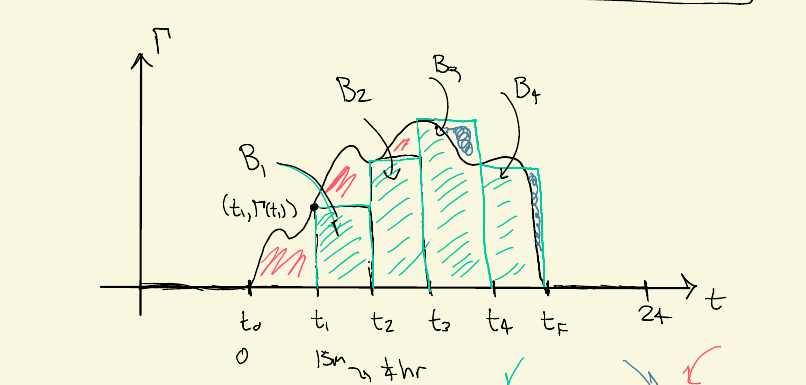
\includegraphics{figures/image_2021-04-18-22-39-08.png}
\caption{image\_2021-04-18-22-39-08}
\end{figure}

\end{remark}

\begin{proposition}[?]

\envlist

\begin{itemize}
\tightlist
\item
  \(f(\theta) \coloneqq\cos(\theta)\) is an even function.
\item
  \(g(\theta) \coloneqq\sin(\theta)\) is an odd function.
\end{itemize}

\end{proposition}

\begin{proof}[?]

Plot vectors for \(\theta, -\theta\) on \(S^1\) and flip over the
\(x{\hbox{-}}\)axis.

\end{proof}

\begin{corollary}[?]

\envlist

\begin{itemize}
\tightlist
\item
  \(\cos(t), \sec(t)\) are even.
\item
  \(\sin(t), \csc(t), \tan(t), \cot(t)\) are odd.
\end{itemize}

\end{corollary}

\hypertarget{wave-function}{%
\subsection{Wave Function}\label{wave-function}}

\begin{remark}

Motivation: let a vector run around the unit circle, where we think of
\(\theta\) as a time parameter. What are its \(x\) and \(y\)
coordinates? What happens if we plot \(x(t)\) in a new \(\theta\) plane?

\end{remark}

\begin{definition}[Standard Form of a Wave Function]

The \textbf{standard form} of a wave function is given by
\begin{align*}
f(t) \coloneqq A \cos(\omega (t - \varphi)) + \delta
,\end{align*}

where

\begin{itemize}
\tightlist
\item
  \(A\) is the \textbf{amplitude},
\item
  \(\omega\) is the \textbf{frequency},
\item
  \(\phi\) is the \textbf{phase shift}, and
\item
  \(\delta\) is the \textbf{vertical shift}.
\item
  \(P \coloneqq 2\pi / \omega\) is the \textbf{period}, so
  \(f(t+kP) = f(t)\) for all \(k\in {\mathbb{Z}}\).
\end{itemize}

\todo[inline]{Insert plot}

\end{definition}

\begin{remark}

Note that this is nothing more than a usual cosine wave, just
translated/dilated in the \(x\) direction and the \(y\) direction.

\end{remark}

\begin{warnings}

Don't memorize equations like \(y=\sin(Bt+C)\) and e.g.~the phase shift
if \(\phi = -C/B\). Instead, use a process: always put your equation in
standard form, then you can just read off the parameters. For example:
\begin{align*}
f(t) 
&= \cos(Bt+C) \\
&= \cos( B (t + {C\over B}) ) \\
&= \cos(\omega (t - \phi) ) \\ \\
&\implies B = \omega, \phi = -{C\over B}
.\end{align*}

\end{warnings}

\begin{example}[?]

Put the following wave in standard form:
\begin{align*}
f(t) \coloneqq 4\cos(3t+2)
.\end{align*}

\end{example}

\begin{example}[?]

Put the following wave in standard form:
\begin{align*}
f(t) \coloneqq\alpha \cos(\beta t+\gamma)
.\end{align*}

\end{example}

\begin{proposition}[?]

How to plot the graph of a wave equation:

\begin{enumerate}
\def\labelenumi{\arabic{enumi}.}
\tightlist
\item
  Put in standard form.
\item
  Read off the parameters to build a rectangular box of width \(P\) and
  height \(2{\left\lvert {A} \right\rvert}\) about the line
  \(y=\delta\).
\item
  Break the box into 4 pieces using the key points
  \(t = \phi + {k\over 4}P\) for \(k=0,1,2,3,4\).
\end{enumerate}

\end{proposition}

\begin{example}[Plotting]

Plot the following function in the \(t\) plane:
\begin{align*}
f(t) = 2 \cos\qty{5t - {\pi \over 2} } + 7
.\end{align*}

\end{example}

\begin{example}[?]

Plot the following:
\begin{align*}
f(t) = -2\sin(3t-7)
.\end{align*}

\end{example}

\begin{proposition}[Determining the equation of a sine wave]

Given a picture of a graph of a sine wave,

\begin{enumerate}
\def\labelenumi{\arabic{enumi}.}
\tightlist
\item
  Draw a horizontal line cutting the wave in half. This will be
  \(\delta\).
\item
  Measure the distance from this midline to a peak. This will be
  \({\left\lvert {A} \right\rvert}\).
\item
  Restrict to one full period, starting either at a peak (if you want to
  match \(\cos(t)\)) or a zero (if you want to match \(\sin(t)\)). Pick
  the period starting as close as possible to the \(y{\hbox{-}}\)axis.
\item
  Measure the period \(P\) and reverse-engineer it to get \(\omega\):
  \(P = 2\pi/\omega \implies \omega = 2\pi/P\).
\item
  Measure the distance from the starting point to the
  \(y{\hbox{-}}\)axis: this is \(\phi\).
\end{enumerate}

\end{proposition}

\begin{example}[?]

Determine the equation of the following wave function:

\begin{figure}
\centering
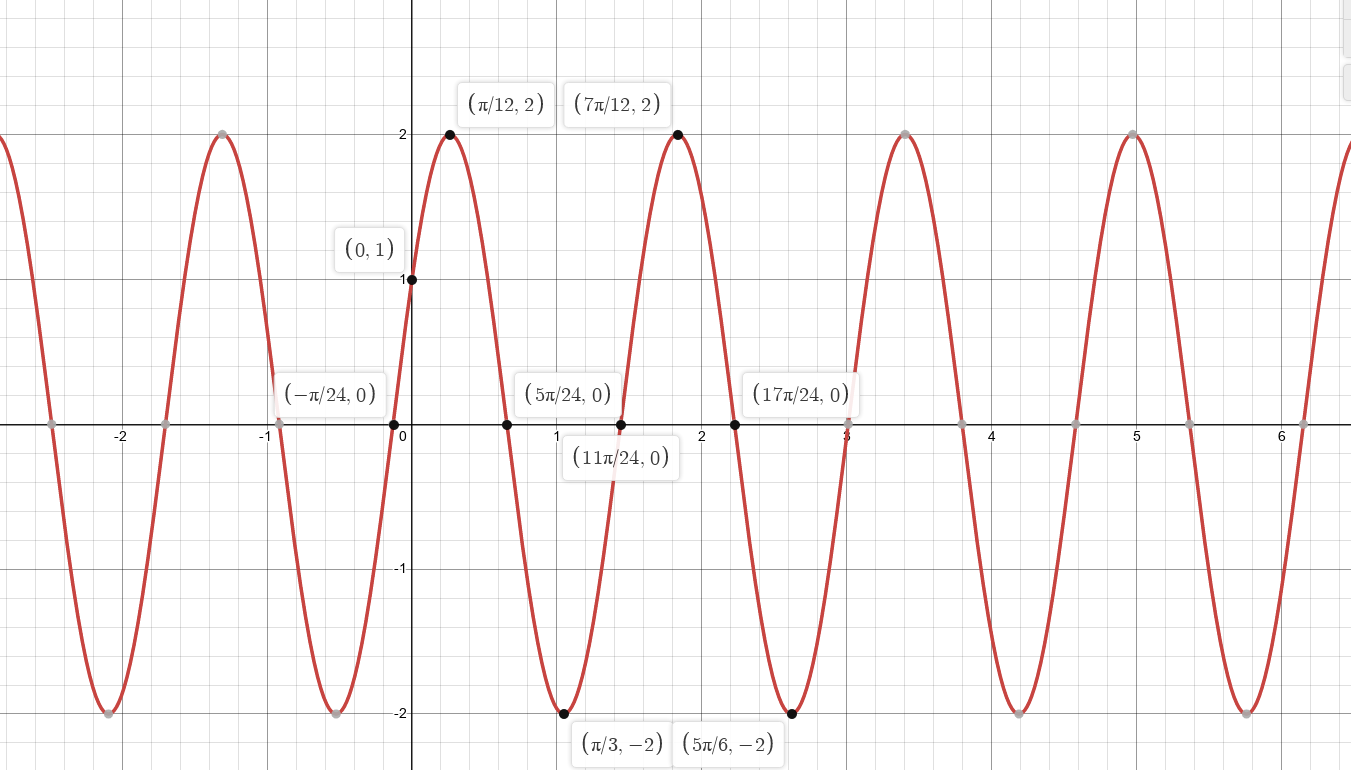
\includegraphics{figures/image_2021-04-18-20-51-34.png}
\caption{image\_2021-04-18-20-51-34}
\end{figure}

\begin{solution}

\begin{align*}
f(t) = 2\sin\qty{4t + {\pi \over 6} }
.\end{align*}

\end{solution}

\end{example}

\begin{remark}

Note that we can graph other trigonometric functions: they get pretty
wild though.

\begin{itemize}
\tightlist
\item
  Tangent: 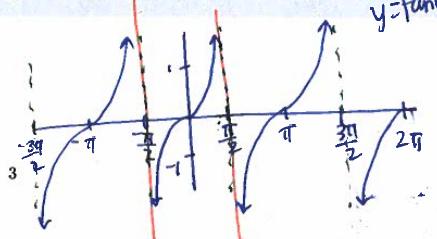
\includegraphics{figures/image_2021-04-18-21-01-06.png}
  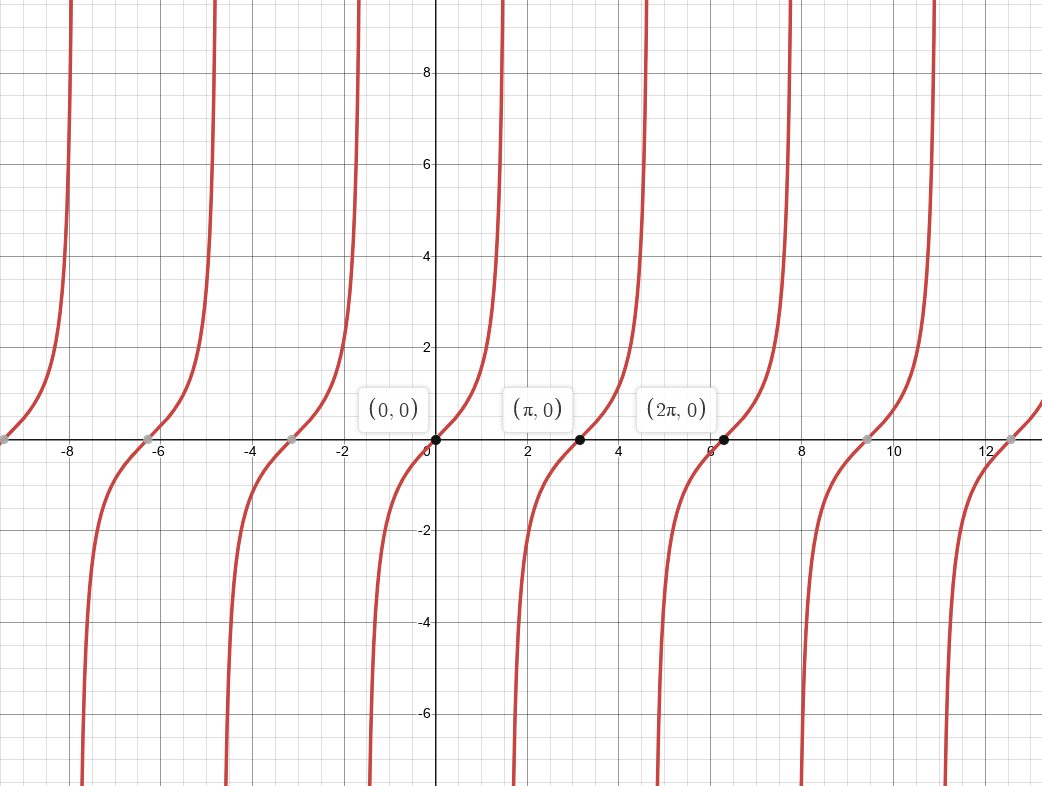
\includegraphics{figures/image_2021-04-18-21-01-38.png}
\end{itemize}

\end{remark}

\hypertarget{inverse-functions}{%
\subsection{Inverse Functions}\label{inverse-functions}}

\begin{remark}

Motivation: we want a way to solve equations where the unknown
\(\theta\) is stuck in the argument of a trigonometric function. For
example, for \(\sin: {\mathbb{R}}_A \to {\mathbb{R}}_B\), this would be
some function \(f: {\mathbb{R}}_B \to {\mathbb{R}}_A\) such that
\begin{align*}
f(\sin(\theta)) &= \operatorname{id}(\theta) = \theta \\
\sin(f(y)) &= \operatorname{id}(y) = y
.\end{align*}

\begin{figure}
\centering
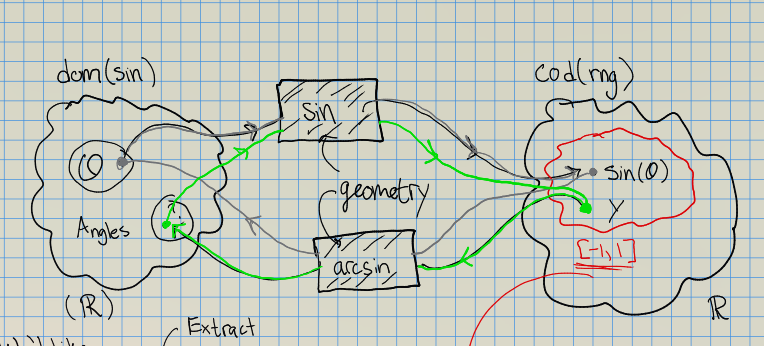
\includegraphics{figures/image_2021-04-18-22-24-55.png}
\caption{image\_2021-04-18-22-24-55}
\end{figure}

Note that we only ever have to define \(f\) on
\(\mathop{\mathrm{range}}(\sin)\), since we're only ever sending outputs
of \(f\) in as the inputs of \(\sin\). So we need
\(\mathop{\mathrm{range}}(\sin) \subset \operatorname{dom}(f)\), noting
that \(\mathop{\mathrm{range}}(\sin) = [-1, 1]\):
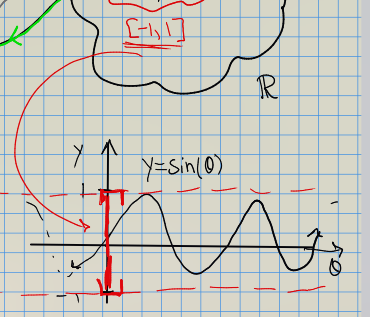
\includegraphics{figures/image_2021-04-18-22-26-56.png}

Similarly, we need
\(\mathop{\mathrm{range}}(f) \subset \operatorname{dom}(\sin)\).

\end{remark}

\begin{remark}

The setup: try swapping \(y\) and \(\theta\) in the graph of
\(y=\sin(\theta)\):

\begin{figure}
\centering
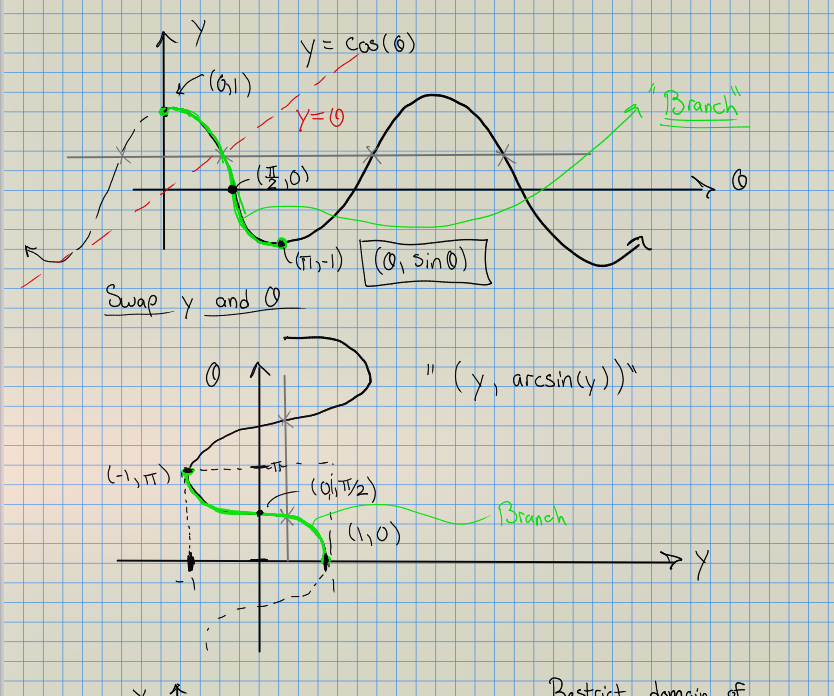
\includegraphics{figures/image_2021-04-18-22-32-36.png}
\caption{image\_2021-04-18-22-32-36}
\end{figure}

Note that the latter is a function (vertical line test) iff the former
is injective (horizontal line test). So we take the largest branch where
the inverse is a function:

\begin{figure}
\centering
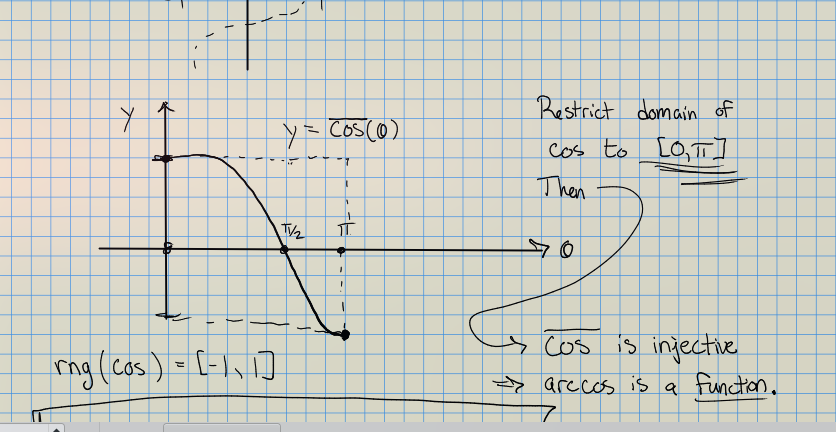
\includegraphics{figures/image_2021-04-18-22-33-27.png}
\caption{image\_2021-04-18-22-33-27}
\end{figure}

Back on our original graph, this looks like the following:

\begin{figure}
\centering
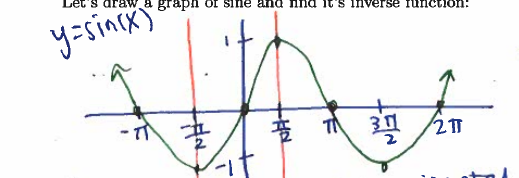
\includegraphics{figures/image_2021-04-18-20-53-25.png}
\caption{image\_2021-04-18-20-53-25}
\end{figure}

Restricting, we get

\begin{itemize}
\tightlist
\item
  \(\operatorname{dom}(\arccos) \coloneqq\mathop{\mathrm{range}}({ \color{green} \cos} ) = [-1, 1]\).
\item
  \(\mathop{\mathrm{range}}(\arccos) \coloneqq\operatorname{dom}( {\color{green} \cos} ) = [0, \pi]\).
\end{itemize}

\end{remark}

\begin{remark}

A similar analysis works for \(\sin(\theta)\):

\begin{figure}
\centering
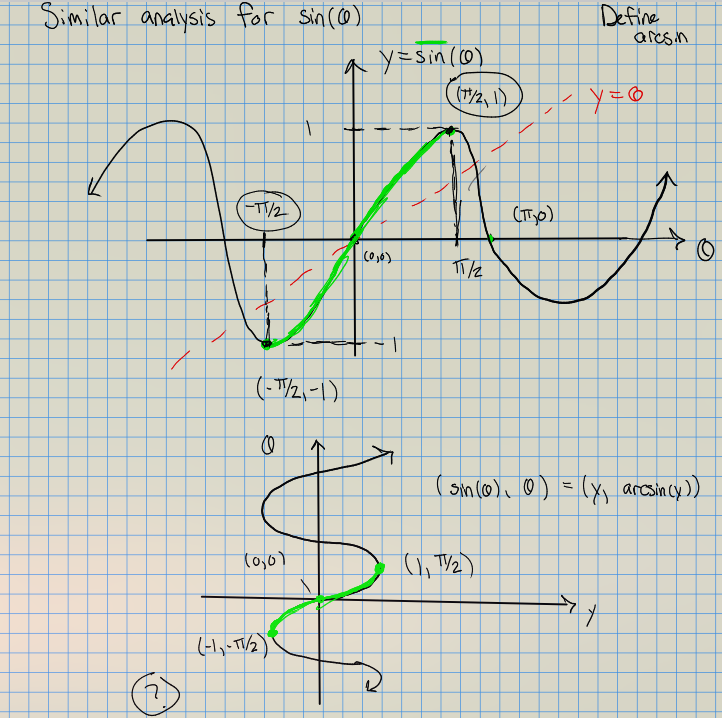
\includegraphics{figures/image_2021-04-18-22-34-21.png}
\caption{image\_2021-04-18-22-34-21}
\end{figure}

Restricting, we get

\begin{itemize}
\tightlist
\item
  \(\operatorname{dom}(\arcsin) \coloneqq\mathop{\mathrm{range}}({ \color{green} \sin} ) = [-1, 1]\).
\item
  \(\mathop{\mathrm{range}}(\arcsin) \coloneqq\operatorname{dom}( {\color{green} \sin }) = [-\pi/2, \pi/2]\).
\end{itemize}

\end{remark}

\begin{remark}

This gives us a new tool to solve equations:
\begin{align*}
\vdots &= \vdots \\
\implies \cos(x) &= b \\
\implies \arccos(\cos(x)) &= \arccos(b) \\
\implies x &= \arccos(b)
,\end{align*}
but only if we know this makes sense based on domain/range issues.

\end{remark}

\begin{proposition}[Domains of inverse trigonometric functions]

Restrict domains in the following ways:

\begin{itemize}
\tightlist
\item
  \(\sin\): \([-\pi/2, \pi/2]\)
\item
  \(\cos: [0, \pi]\)
\item
  \(\tan: [-\pi/2, \pi/2]\)
\end{itemize}

\begin{longtable}[]{@{}
  >{\raggedright\arraybackslash}p{(\columnwidth - 4\tabcolsep) * \real{0.20}}
  >{\raggedright\arraybackslash}p{(\columnwidth - 4\tabcolsep) * \real{0.61}}
  >{\raggedright\arraybackslash}p{(\columnwidth - 4\tabcolsep) * \real{0.17}}@{}}
\toprule
Function & Domain & Range \\
\midrule
\endhead
\(\arcsin\) & \([-1, 1]\) & \([-\pi/2, \pi /2]\) \\
\(\arccos\) & \([-1, 1]\) & \([0, \pi]\) \\
\(\arctan\) & \({\mathbb{R}}\) & \((-\pi/2, \pi/2)\) \\
\(\operatorname{arccsc}\) &
\({\mathbb{R}}\setminus\left\{{0, \pm {\pi}, \pm{2\pi}, \cdots}\right\}\)
& ? \\
\(\operatorname{arcsec}\) &
\({\mathbb{R}}\setminus\left\{{\pm {\pi \over 2}, \pm{3\pi \over 2}, \cdots}\right\}\)
& ? \\
\(\operatorname{arccot}\) &
\({\mathbb{R}}\setminus\left\{{0, \pm {\pi}, \pm{2\pi}, \cdots}\right\}\)
& ? \\
\bottomrule
\end{longtable}

\end{proposition}

\begin{example}[?]

We have some exact values.

Sines should be in QI or QIV:

\begin{itemize}
\tightlist
\item
  \(\arcsin(1/2) = \pi/6\)
\item
  \(\arcsin(\sqrt{3}/2) = \pi/3\)
\item
  \(\arcsin(-1/2) = -\pi/6\)
\end{itemize}

Cosines should be in QI or QII:

\begin{itemize}
\tightlist
\item
  \(\arccos(\sqrt{3}/2) = \pi/6\)
\item
  \(\arccos(-\sqrt{2}/2) = 3\pi/4\)
\item
  \(\arccos(1/2) = \pi/3\)
\end{itemize}

Tangents should be in QI or QIV:

\begin{itemize}
\tightlist
\item
  \(\arctan(\sqrt{3}/3) = \pi/6\)
\item
  \(\arctan(0) = 0\)
\item
  \(\arctan(1) = \pi/4\)
\end{itemize}

\end{example}

\begin{warnings}

Note that if \(f, g\) are an inverse pair, we have
\begin{align*}
f\circ g = \operatorname{id}\quad\iff\quad f(g(x)) = x,\quad g(f(x)) = x
.\end{align*}
However, we have to be careful with domains for trigonometric functions:

\begin{itemize}
\tightlist
\item
  \(\arcsin(\sin(x)) = x \iff x\in [-\pi/2, \pi/2]\) (restricted domain
  of \(\sin\))
\item
  \(\sin(\arcsin(x)) = x \iff x\in [-1, 1]\) (domain of \(\arcsin\))
\item
  \(\arccos(\cos(x)) = x \iff x\in [0, \pi]\) (restricted domain of
  \(\cos\))
\item
  \(\cos(\arccos(x)) = x \iff x\in [-1, 1]\) (domain of \(\arccos\))
\item
  \(\arctan(\tan(x)) = x \iff x\in [0]\) (restricted domain of \(\tan\))
\item
  \(\tan(\arctan(x)) = x \iff x\in {\mathbb{R}}\)

  \begin{itemize}
  \tightlist
  \item
    Domain of \(\arctan\), then range is \([-\pi/2, \pi/2]\), which is
    in the domain of \(\tan\).
  \end{itemize}
\end{itemize}

\end{warnings}

\begin{remark}

Most inverse trigonometric functions can \emph{not} be exactly solved!
We'll have to approximate by calculator if we want the actual angle. If
we just want \emph{other} trigonometric functions though, we can always
embed in a triangle.

\end{remark}

\begin{example}[?]

Show the following:

\begin{itemize}
\tightlist
\item
  \(\cos(\arcsin(24/26)) = 10/26\)

  \begin{itemize}
  \tightlist
  \item
    Write \(\theta = \arcsin(24/26)\), note \(\theta\) is in
    \([-\pi/2, \pi/2] = \mathop{\mathrm{range}}(\arcsin)\).
  \end{itemize}
\item
  \(\tan(\arccos(-10/26)) = 10/26\)

  \begin{itemize}
  \tightlist
  \item
    Write \(\theta = \arccos(-10/26)\), note \(\theta\) is in
    \([0, \pi] = \mathop{\mathrm{range}}(\arccos)\)
  \end{itemize}
\end{itemize}

\end{example}

\begin{exercise}[?]

Compute \(\arcsin(3/5)\).

\end{exercise}

\begin{warnings}

This is equal to \(\sin^{-1}(3/5)\), which is \emph{not} equal to
\({1\over \sin(3/5)}\)! One way to remember this is that we have another
name for reciprocals, here \(\csc(3/5)\).

\end{warnings}

\begin{solution}

\begin{align*}
\theta &= \arcsin(3/5) \\
\implies \sin(\theta) = (3/5) && \text{roughly by injectivity} \\
\implies &\cdots ?
.\end{align*}
We are out of luck, since this isn't a special angle. So we can't find a
numerical value of \(\theta\). We can find other trig functions of
\(\theta\) though:

\begin{figure}
\centering
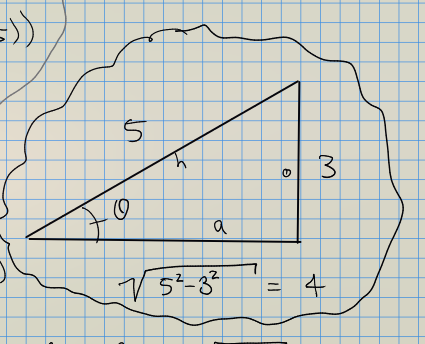
\includegraphics{figures/image_2021-04-18-22-30-09.png}
\caption{image\_2021-04-18-22-30-09}
\end{figure}

So for example, \(\cos(\arcsin(3/5)) = 4/5\).

\end{solution}

\hypertarget{simplifying-identities}{%
\subsection{Simplifying Identities}\label{simplifying-identities}}

\begin{remark}

The goal: reduce a complicated mess of trigonometric functions to
something as simple as possible. We'll use a \textbf{boxing-up method}.

\end{remark}

\begin{exercise}[?]

Simplify the following:
\begin{align*}
F(\theta) \coloneqq\qty{ \sin(\theta) \cos(\theta) \over \cot(\theta)} \cos(\theta)\csc(\theta)
.\end{align*}

\end{exercise}

\begin{solution}

\begin{align*}
F = s \qty{s \over c}
.\end{align*}

\end{solution}

\begin{remark}

On verifying identities: if you want to show \(f(\theta) = g(\theta)\),
start at one and arrive at the other:
\begin{align*}
f(\theta) &= \text{simplify } f \\
&= \cdots \\
&= \cdots \\
&= \cdots \\
&= g(\theta) \\
.\end{align*}

\end{remark}

\begin{warnings}

If you end up with something like \(1=1\) or \(0=0\), this is hinting at
a problem with your logic.

\end{warnings}

\begin{remark}

As an alternative, you can use the \textbf{transitivity of equality}:
show that \(f(\theta) = h(\theta)\) for some totally different function
\(h\), and then show \(g(\theta) = h(\theta)\) as well.

\begin{figure}
\centering
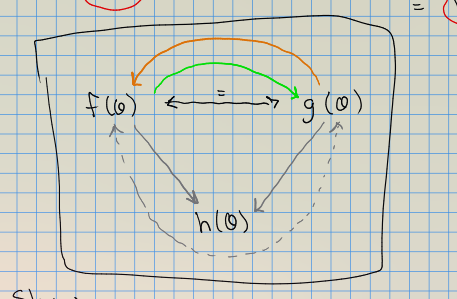
\includegraphics{figures/image_2021-04-18-21-58-52.png}
\caption{image\_2021-04-18-21-58-52}
\end{figure}

\end{remark}

\begin{example}[?]

Show the following identity:
\begin{align*}
{\sin(-\theta) + \csc(\theta)} = \cot(\theta) \cos(\theta)
\end{align*}
by showing both sides are separately equal to
\(h(\theta) \coloneqq\csc(\theta) - \sin(\theta)\).

\end{example}

\hypertarget{doublehalf-angle-identities}{%
\subsection{Double/Half-Angle
Identities}\label{doublehalf-angle-identities}}

\begin{remark}

Sometimes we are interested in \textbf{superposition} of waves.
Mathematically this is modeled by multiplying two wave functions
together. We can sometimes rewrite these as a \emph{single} wave with a
phase shift.

\end{remark}

\begin{proposition}[?]

Identities:
\begin{align*}
\sin(\theta + \psi) &= \sin(\theta) \cos(\psi) + \cos(\theta) \sin(\psi) \\
\cos(\theta + \psi) &= \cos(\theta) \cos(\psi) + \sin(\theta) \sin(\psi)
.\end{align*}
Note that you can divide these to get
\begin{align*}
\tan(\theta + \psi) &= {\tan(\theta) + \tan(\psi) \over 1 - \tan(\theta) \tan(\psi) }
,\end{align*}
and replace \(\psi\) with \(-\psi\) and use even/odd properties to get
formulas for \(\sin(\theta - \psi), \cos(\theta - \psi)\)

\end{proposition}

\begin{slogan}

Sines are friendly and cosines are clique-y!

\end{slogan}

\begin{remark}

The most interesting modifications of waves: superpositions and damped
waves.

\begin{figure}
\centering
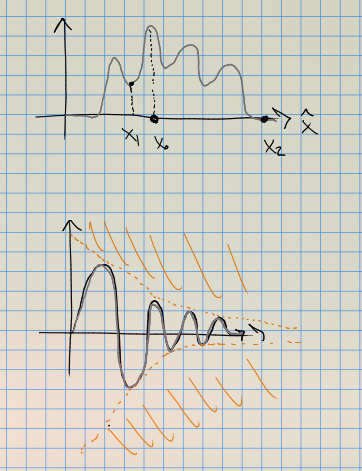
\includegraphics{figures/image_2021-04-18-22-06-08.png}
\caption{image\_2021-04-18-22-06-08}
\end{figure}

\end{remark}

\begin{corollary}[Double angle identities]

Taking \(\theta = \psi\) is the above identities yields
\begin{align*}
\sin(2\theta ) 
&= \sin(\theta) \cos(\theta) + \cos(\theta) \sin(\theta) \\
&= 2\sin(\theta)\cos(\theta) \\ \\
\cos(2\theta) 
&= \cos(\theta) \cos(\theta) + \sin(\theta) \sin(\theta) \\
&= \cos^2(\theta) - \sin^2(\theta) 
.\end{align*}

\end{corollary}

\begin{warnings}

The latter is not equal to 1! That would be
\(\cos^2(\theta) + \sin^2(\theta)\).

\end{warnings}

\begin{remark}

Why do we care? We had 16 special angles, this gives a lot more. For
example,
\begin{align*}
\cos(\pi/12)
=
\cos(\pi/3 - \pi/4) = \cdots \text{ plug in}
.\end{align*}
By allowing increments of \(\pi/12\), we have 24 total angles.

\end{remark}

\begin{corollary}[?]

Starting from the following:
\begin{align*}
\cos(2\theta) 
&= \cos^2(\theta) - \sin^2(\theta) \\
&= \cos^2(\theta) - \qty{1 - \cos^2(\theta) } \\
&= 2\cos^2(\theta) -1 && \text{using } s^2 + c^2 = 1
,\end{align*}
one can solve for
\begin{align*}
\cos^2(\theta) = {1\over 2}\qty{1 + \cos(2\theta) }
.\end{align*}

Similarly
\begin{align*}
\cos(2\theta) 
&= \cos^2(\theta) - \sin^2(\theta) \\
&= \qty{1 - \sin^2(\theta) } - \sin^2(\theta) \\
&= 1-2\sin^2(\theta) && \text{using } s^2 + c^2 = 1
,\end{align*}
solving yields
\begin{align*}
\sin^2(\theta) = {1\over 2} (1 - \cos(2\theta) )
.\end{align*}

\end{corollary}

\hypertarget{bonus-complex-exponentials}{%
\subsection{Bonus: Complex
Exponentials}\label{bonus-complex-exponentials}}

\begin{remark}

Components of vectors: every \(\mathbf{v}\in {\mathbb{R}}^2\) breaks up
as the sum of two vectors,
i.e.~\(\mathbf{v} = \mathbf{v}_x + \mathbf{v}_y\).

\end{remark}

\begin{remark}

We've worked with the \emph{Cartesian plane} all semester. One powerful
tool is replacing this with the \emph{complex} plane. We formally define
a new symbol \(i\) such that \(i^2 = -1\), and replace the
\(\widehat{ \mathbf{y} }\) direction with the \(i\) direction -- this
amounts to replacing ordered pairs
\((a, b) \coloneqq a \widehat{ \mathbf{x} } + b\widehat{ \mathbf{y} }\)
by a single number \(x + iy\).

\end{remark}

\begin{proposition}[Euler's Identity]

\begin{align*}
e^{i\pi} = -1
.\end{align*}

\end{proposition}

\begin{remark}

The way you read this: \(e^{i\theta} \in S^1\) is a complex number
(identified with a vector!), and the \(\theta\) tells you what direction
it points in radians. \(\pi\) radians is directly to the left!

\end{remark}

\addsec{ToDos}
\listoftodos[List of Todos]
\cleardoublepage

% Hook into amsthm environments to list them.
\addsec{Definitions}
\renewcommand{\listtheoremname}{}
\listoftheorems[ignoreall,show={definition}, numwidth=3.5em]
\cleardoublepage

\addsec{Theorems}
\renewcommand{\listtheoremname}{}
\listoftheorems[ignoreall,show={theorem,proposition}, numwidth=3.5em]
\cleardoublepage

\addsec{Exercises}
\renewcommand{\listtheoremname}{}
\listoftheorems[ignoreall,show={exercise}, numwidth=3.5em]
\cleardoublepage

\addsec{Figures}
\listoffigures
\cleardoublepage


\printbibliography[title=Bibliography]


\end{document}
